\documentclass[hyperref={pdfpagelabels=false}]{beamer}
\setbeamercolor{background canvas}{bg=white}
\usepackage{graphicx,lmodern,subfigure,ulem,color,graphicx,tikz,booktabs,natbib}
%\usepackage{subfig}
\usepackage{mathrsfs}
\usepackage{subfigure}
\usetheme{Warsaw}
%\definecolor{beamer@blendedblue}{rgb}{0.1,0.5,0.1}
%\definecolor{ForestGreen}{RGB}{60, 140, 60}
%\setbeamercolor{structure}{fg=beamer@blendedblue}
\setbeamertemplate{navigation symbols}{}
\setbeamertemplate{footline}[frame number]
\bibliographystyle{chicago}
\newcommand{\spitem}{\vspace{.3cm}\item}
\newcommand{\elas}{$E_{labor}$}
%\def \FigPath {Users\th3\Documents\Job_Market_Paper\Code\Figures} 
\DeclareMathOperator{\E}{\mathbb{E}}
\usepackage{makecell}




\title{ICT-Specific Investment Shocks and Economic Fluctuations \bigskip \\ \normalsize{Evidence and Theory of a General-Purpose Technology}}
\author{Marco Brianti, Boston College\\Laura G\'ati, Boston College}
\institute{Convegno RECent\\Modena}
\date{\textit{March 2019}}

\usetheme[
outer/progressbar=foot,
outer/numbering=none
]{metropolis}


\begin{document}
	
	\frame{\titlepage}
	

	
		\frame{\frametitle{Motivation}

\bigskip
			
	\textbf{Empirical Fact.} U.S. output has expanded only slowly in the aftermath of the financial crisis
	
	\
	
	Fernald, Hall, Stock and Watson (2017) empirically show that two components explain nearly all this growth gap
	\begin{enumerate}
		\item Slow growth in total factor productivity (TFP)
		\item Falling labor force participation
	\end{enumerate}

\


In this paper we focus on the \textbf{slowdown in TFP},
\begin{itemize}
	\item[$\Rightarrow$] Which variable boosted productivity in the last three decades? 
\item[$\Rightarrow$] Can this variable explain its recent slowdown?
\end{itemize}


	}

	\frame{\frametitle{An alternative to R\&D Investment}	
		
		
		Several papers endogenize TFP through \textbf{R\&D investment}
		\begin{itemize}
			\item Financial crisis $\Rightarrow$ $\downarrow$ $Y$ $\Rightarrow$ $\downarrow$ R\&D $\Rightarrow$ $\downarrow$ TFP 
		\end{itemize}
		
		
		\
		
		However, as showed by Oliner et al. (2007) and Jorgenson et al. (2008), TFP have started slowing down \textbf{before} the crisis.
		\begin{itemize}
			\item[$\Rightarrow$] R\&D cannot be the full story
		\end{itemize}
	
	\
	
	We follow an alternative avenue and focus on the relation between \textbf{Information and Communication Technology Investment} (ICTI) and total factor productivity
	\begin{itemize}
			\item \textit{Acquisition of equipment and computer software meant to be used in production for more than a year.}
			\end{itemize}
		

	
}

\frame{\frametitle{This Paper}

\bigskip
	
	\begin{enumerate}
		\item We identify ICT investment shocks using \textbf{SVAR} techniques
		\begin{itemize}
			\item A contemporaneous increase in ICT investment leads to a delayed, persistent, and large rise in productivity
             \item Historical decomposition confirms that the dot-com crash explains most of the slowdown in TFP since 2006 
		\end{itemize}
	
	\
	
	\
		
		\item We analyze a \textbf{general equilibrium model} to rationalize our empirical findings 
		\begin{itemize}
		\item Our identified shocks can be interpreted as supply shocks specific to the ICT sector
         \item ICT capital boosts productivity of ICT users through a positive externality
\begin{itemize}
\item[$\Rightarrow$] The effectiveness of ICT depends on its own level of diffusion
\end{itemize}
		\end{itemize}
	\end{enumerate}





}
	
	
	\frame{\frametitle{Empirical Analysis}	
		

	We estimate a structural VAR using aggregate quarterly US data from 1989Q1 to 2017Q2. 

\begin{equation}
X_t = B(L)X_{t-1} + \underbrace{A \varepsilon_t}_{u_t}
\end{equation}


\begin{itemize}
	\item $X_t = [ TFP_t   \ \ ICTI_t   \ \ 	RP_t \ \ Y_t ]$ where $RP_t = \pi^{IT}_t/\pi^{CPI}_t$
	\item $Y_t$ represents the log transformations of endogenous variables
	\item A is Cholesky decomposition of $\Sigma_u = u_t' u_t$
\end{itemize}	

\

Focus is on the second structural shock $\varepsilon_{2,t}$ 
\begin{itemize}
	\item[$\Rightarrow$] $\varepsilon_{2,t}$ maximizes the impact effect on $ICTI_t$ and is orthogonal to contemporaneous innovations in TFP
\end{itemize}

	
	}

	\frame{
\frametitle{Impulse Response of TFP to $\varepsilon_{2,t}$}

\begin{figure}[h!]
	\begin{center}
		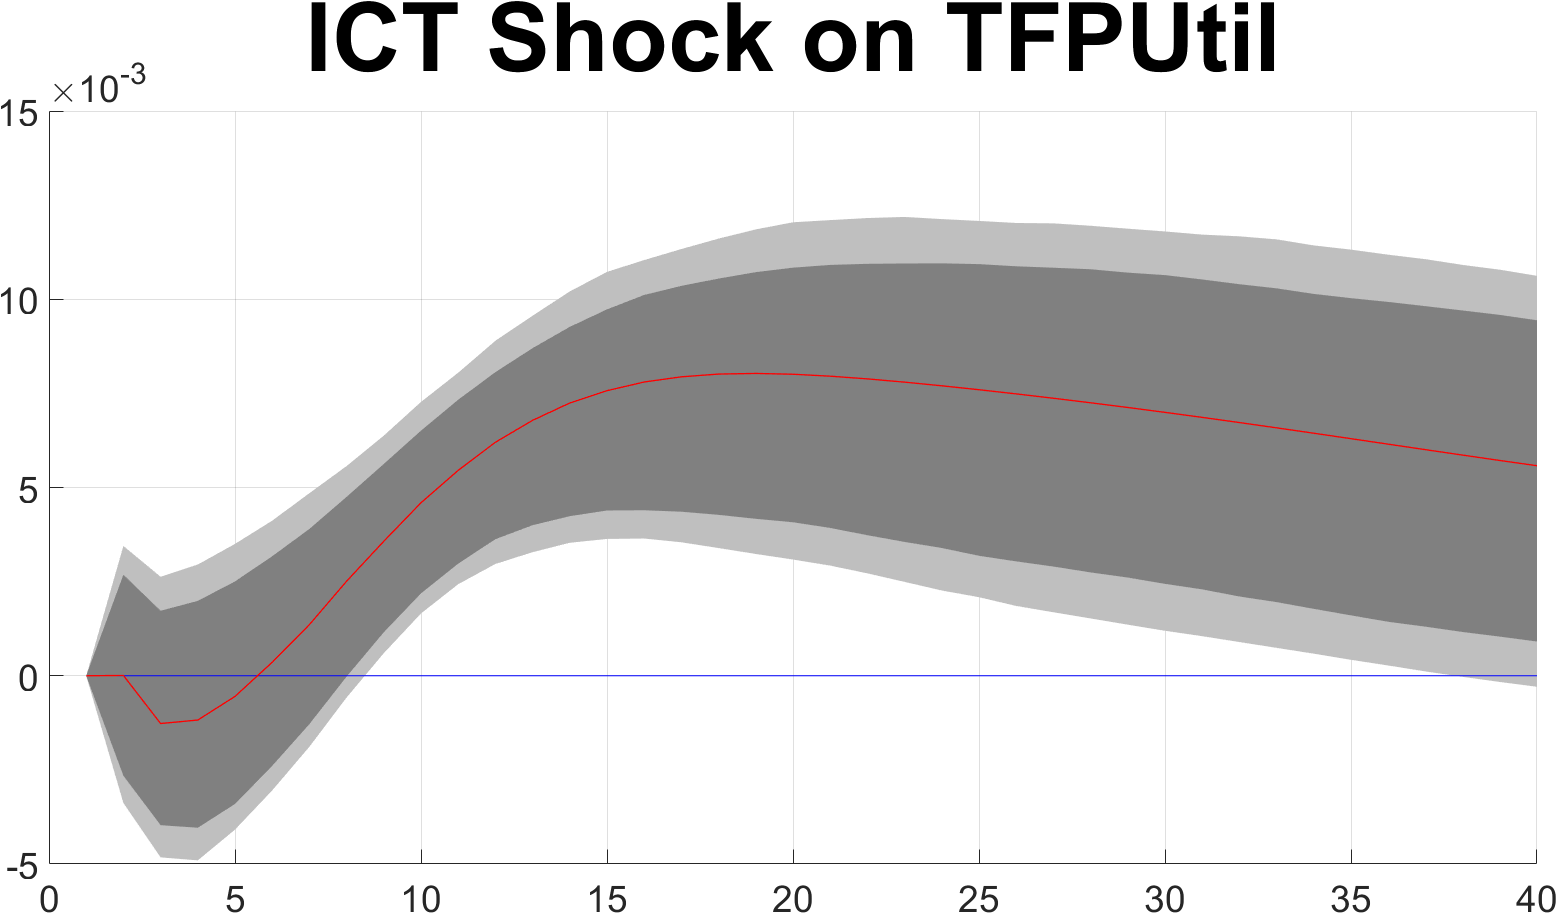
\includegraphics[scale=0.25]{fig_ICT_Shock_on_TFPUtil_empirical_fullEconomy}
		\label{fig:TFP_main}
	\end{center}
\end{figure}
}




\frame{
	\frametitle{Impulse Responses of $X_t$ to $\varepsilon_{2,t}$}

\bigskip

\begin{columns}[t]
\column{.3\textwidth}
\centering
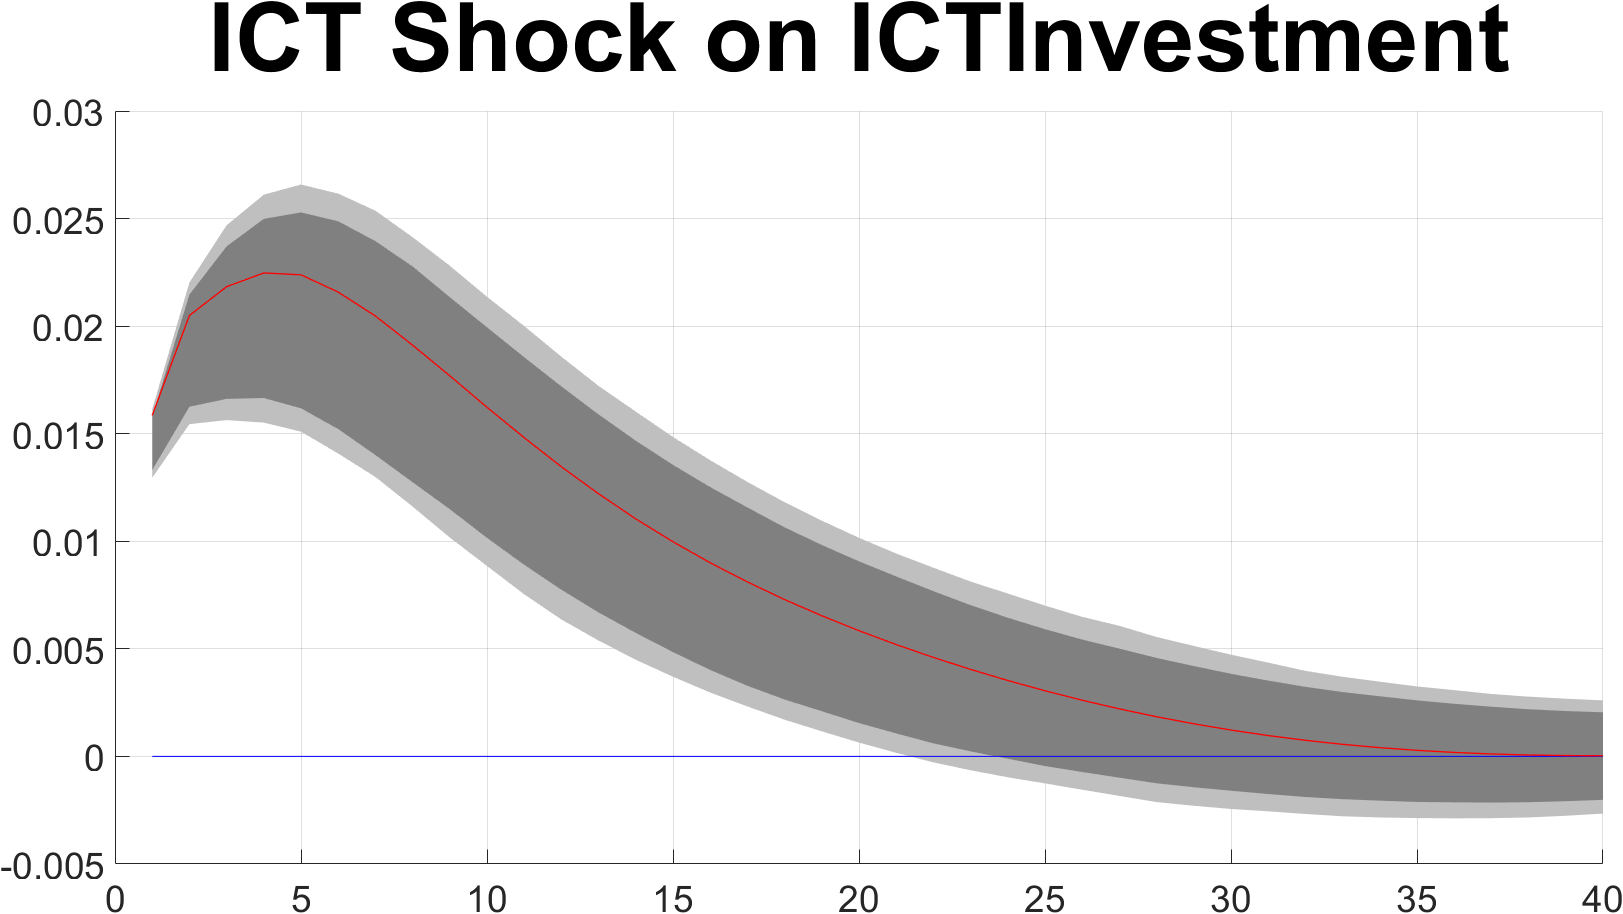
\includegraphics[width=3.5cm,height=3.5cm]{fig_ICT_Shock_on_ICTInvestment_empirical_fullEconomy}\\
\bigskip
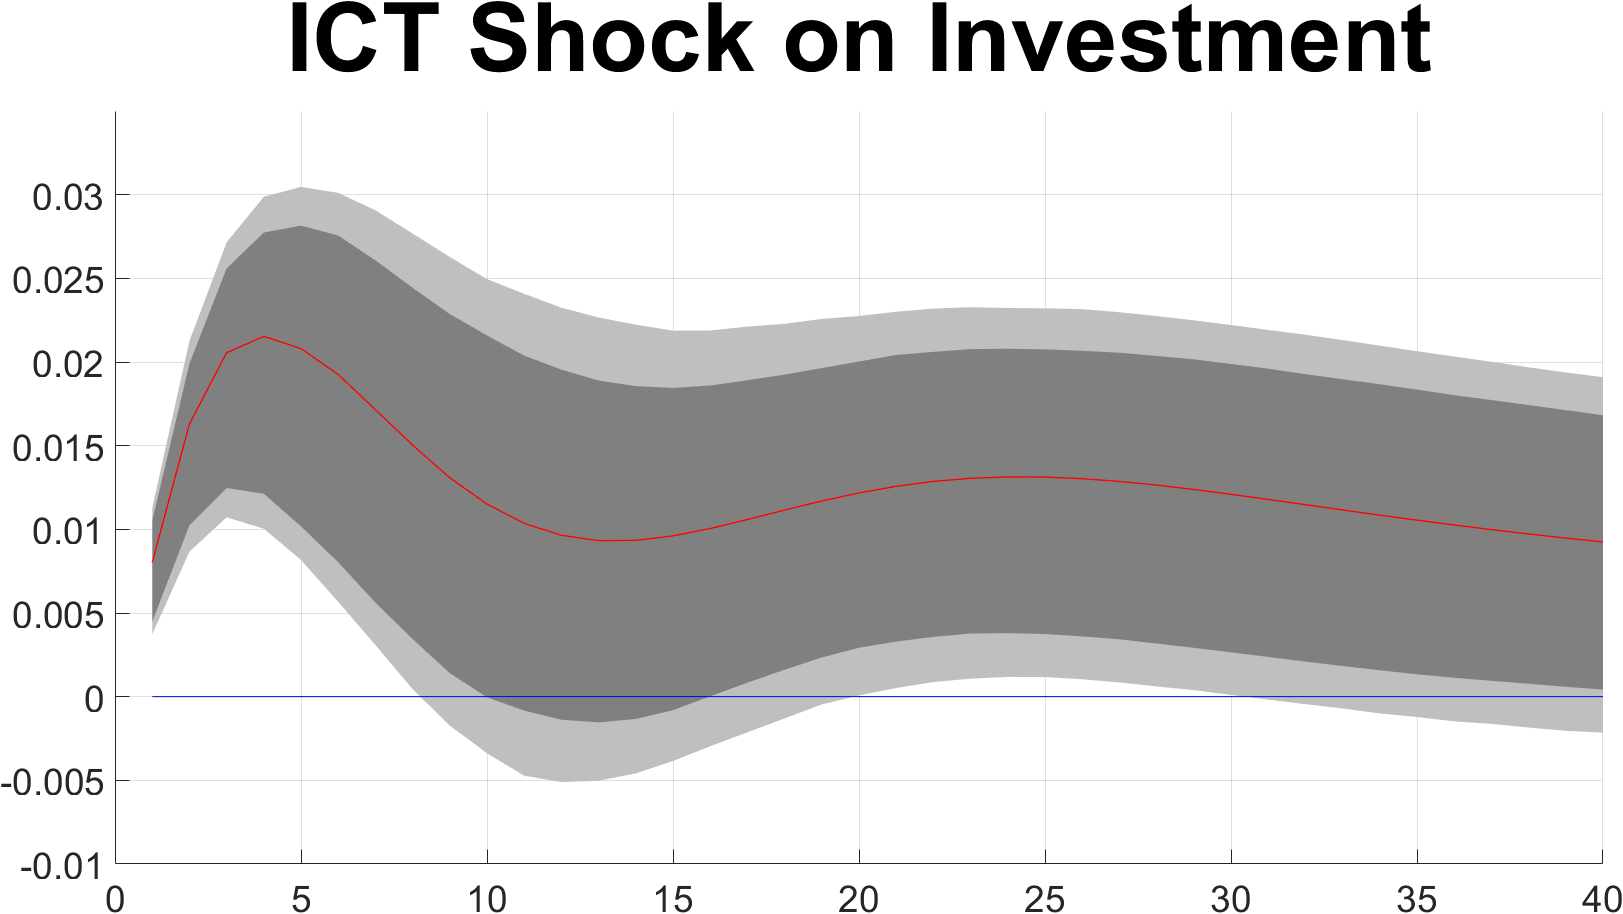
\includegraphics[width=3.5cm,height=3.5cm]{fig_ICT_Shock_on_Investment_empirical_fullEconomy} 
\column{.3\textwidth}
\centering
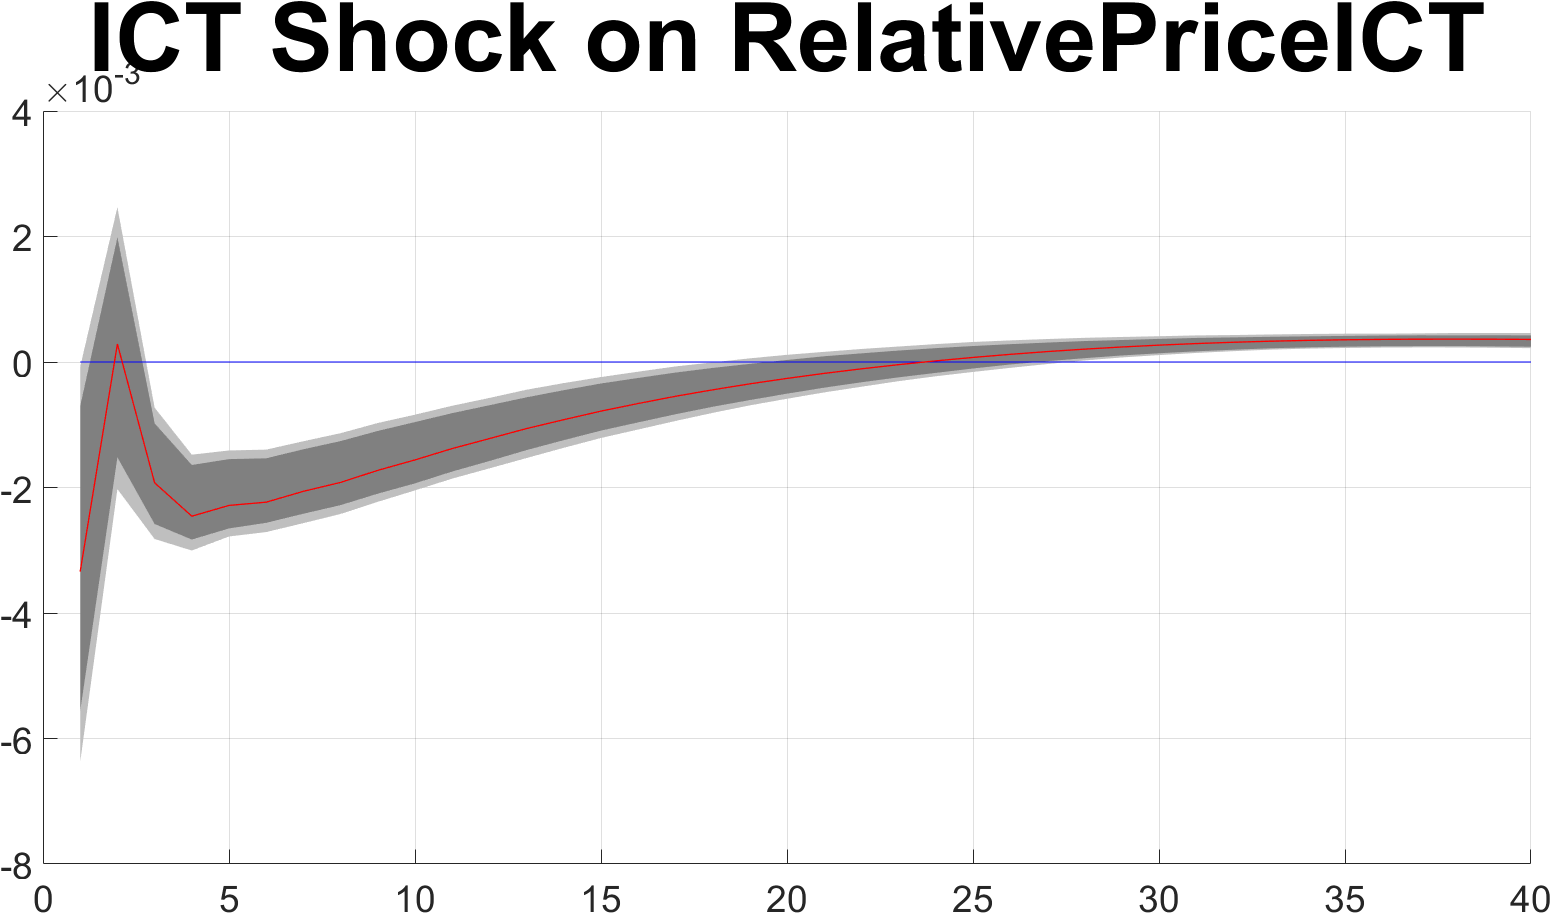
\includegraphics[width=3.5cm,height=3.5cm]{fig_ICT_Shock_on_RelativePriceICT_empirical_fullEconomy}\\
\bigskip
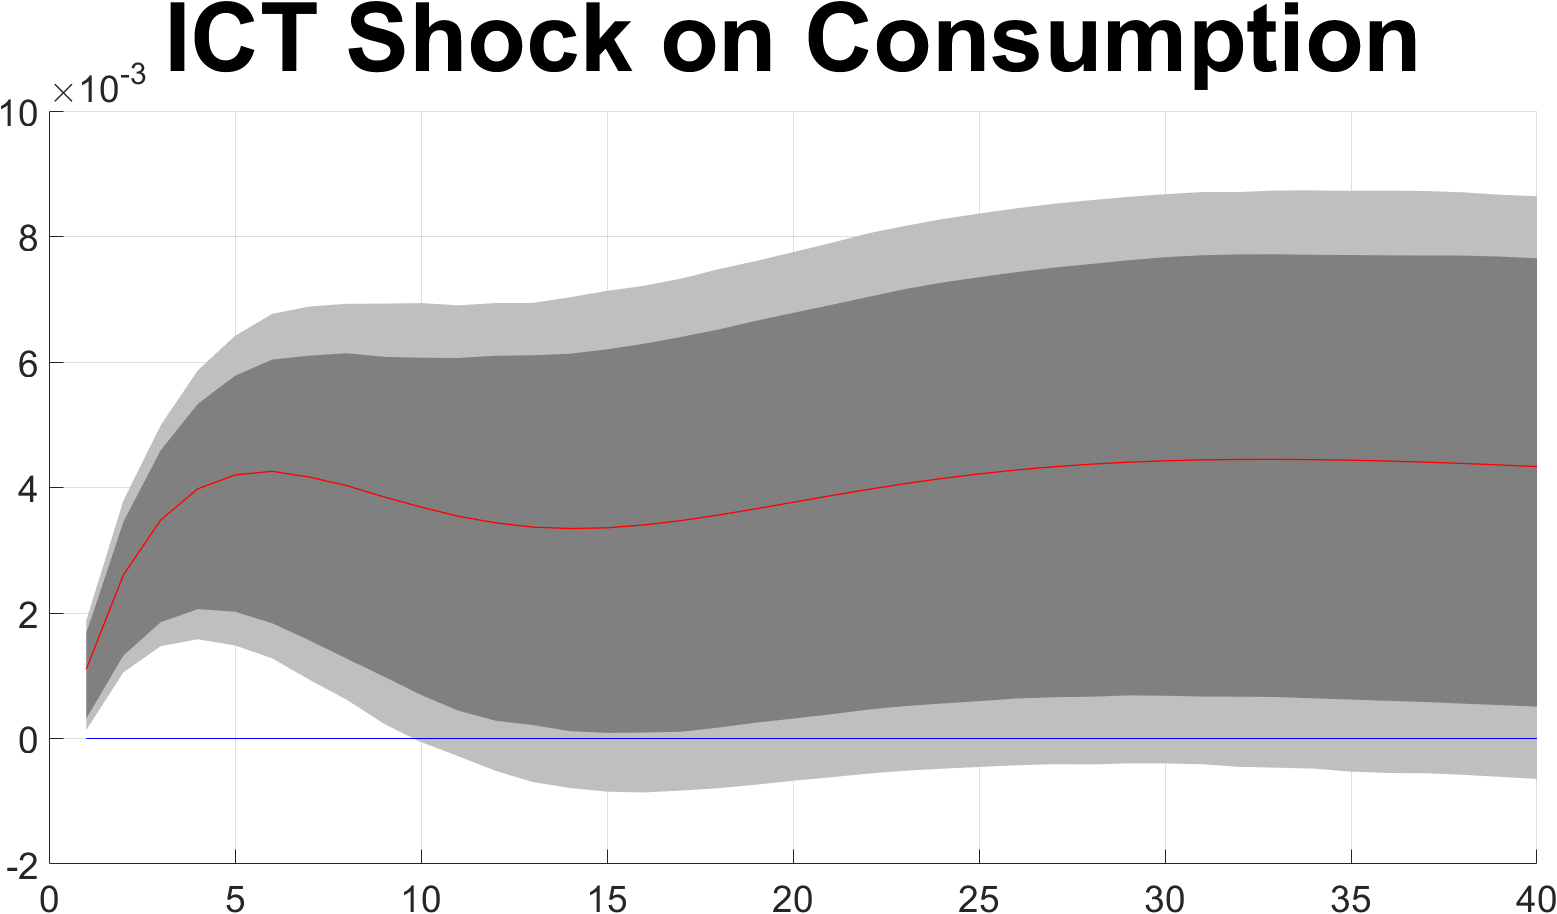
\includegraphics[width=3.5cm,height=3.5cm]{fig_ICT_Shock_on_Consumption_empirical_fullEconomy}
\column{.3\textwidth}
\centering
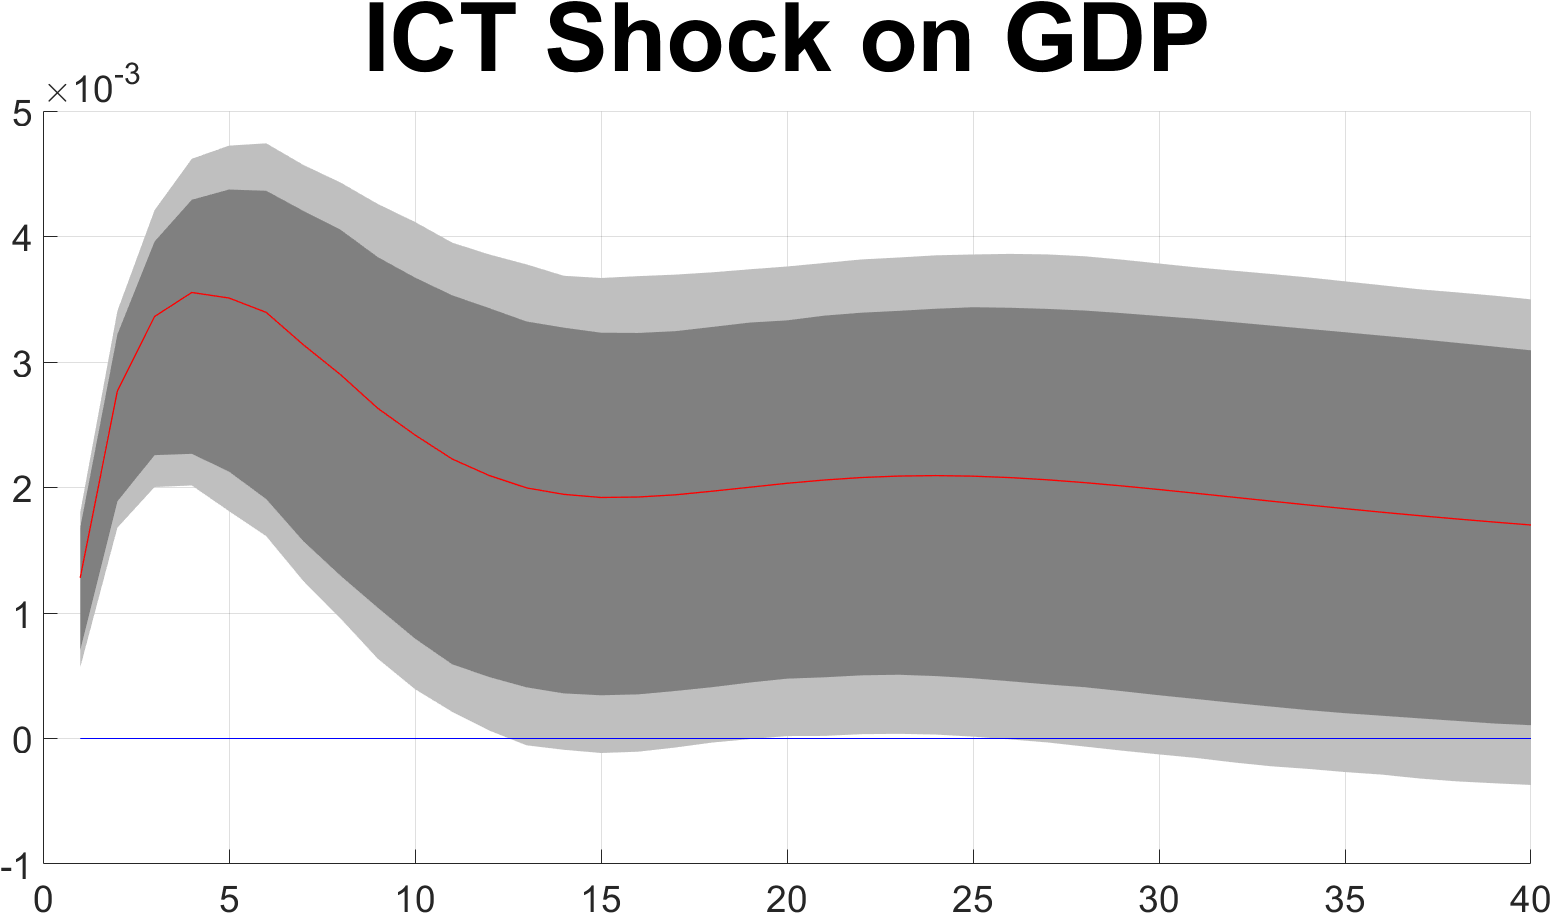
\includegraphics[width=3.5cm,height=3.5cm]{fig_ICT_Shock_on_GDP_empirical_fullEconomy}\\
\bigskip
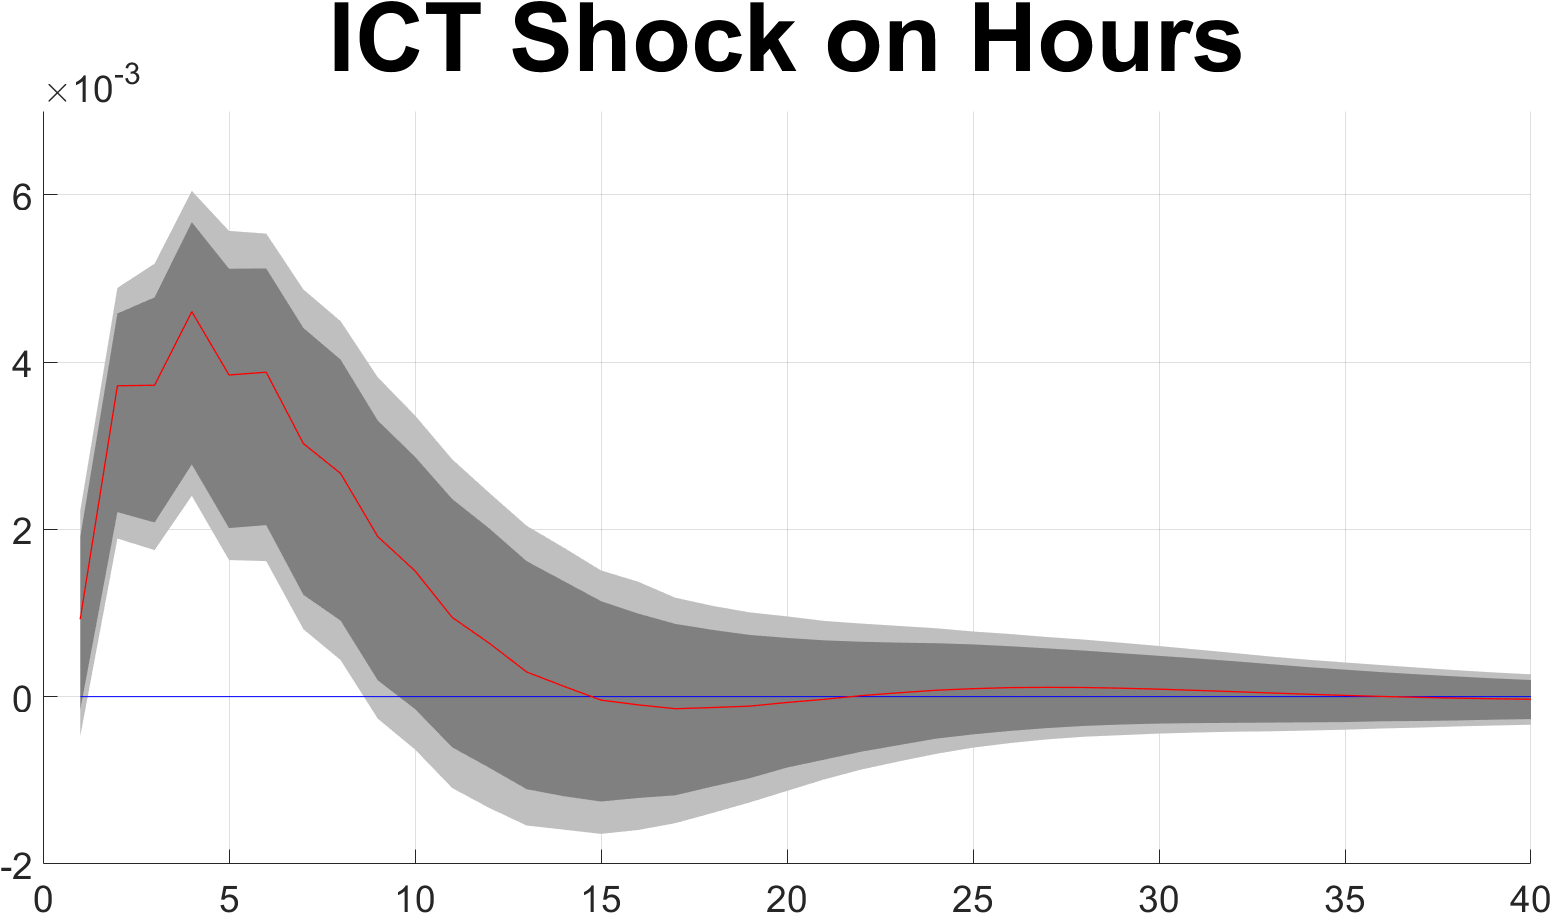
\includegraphics[width=3.5cm,height=3.5cm]{fig_ICT_Shock_on_Hours_empirical_fullEconomy}
\end{columns}



}

	

\frame{\frametitle{Related Exercises and Robustness Checks}

\bigskip
	
	\begin{itemize}
		\item \textbf{Variance Decomposition Analysis}
	\begin{itemize}
		\item[-] Around $30$\% of TFP fluctuations over 10-year horizon 
		\item[-] Almost $40$\% of GDP fluctuations over BC frequencies
	\end{itemize}
\item[$\Rightarrow$]  ICT shocks are an \textbf{important driver} of economic fluctuations


\

\item \textbf{Historical Decomposition Analysis}
\begin{itemize}
\item[-] Large negative shocks in 2000-2001 (dot-com crash) explain the slowdown in TFP since 2006
\end{itemize}
\item[$\Rightarrow$] ICT shocks \textbf{rationalize} the facts by Fernald et al. (2017)


\

\item \textbf{Rebustness Checks} 
\begin{itemize}
	\item[-] Controlling for news shocks \`a la Barsky and Sims
	\item[-] Controlling for other shocks estimated via narrative approach
\end{itemize}
\item[$\Rightarrow$]  ICT shocks are \textbf{not confounded} with other shocks
\end{itemize}

}




\frame{\frametitle{Model}



Main objectives of theoretical analysis
\begin{itemize}
\item[1.] Providing structural interpretation to the identified shocks
\begin{itemize}
\item[$\Rightarrow$] ICT shocks move price and quantities in different directions
\end{itemize}
\item[2.] Rationalize the relation between current ICT investment and future TFP
\begin{itemize}
\item[$\Rightarrow$] Why current ICT investment drives future TFP?
\end{itemize}
\end{itemize}

\

We extend and analyze a 2-sector GE model in the spirit of Greenwood et al. (2000). Two main assumptions are in place,
\begin{itemize}
\item[1.] Second sector specifically produces ICT durable goods to be used as inputs in both sectors' production function
\item[2.] Agents fail to internalize that productivity of both sectors positively depends of the overall ICT diffusion in the economy
\end{itemize}



}

\frame{\frametitle{Main Equations}


Consumption-good sector
\begin{eqnarray}\label{equation:production_FINAL}
y^c_t(j) = A^c_t \ \big( k^c_{t}(j) \big)^a \ \big( k^i_{t}(j) \big)^b \ \big( l_{t}(j) \big)^{1-a-b}
\end{eqnarray}

\

ICT-good sector
\begin{eqnarray}\label{equation:productionICT}
y^i_t(q) = A_t^i \ \big( k^c_{t}(q) \big)^a \ \big( k^i_{t}(q) \big)^b \ \big( l_{t}(q) \big)^{1-a-b}
\end{eqnarray}

\

where

\centering
$ A_t^c = \eta_t \ \theta^c_t \ \textcolor{red}{(k^i_{t})^{\gamma}} \ \ \ \text{and} \ \ \ A_t^i = \eta_t \ \theta^i_t \ \textcolor{red}{(k^i_{t})^{\gamma}} $	





}
		


\frame{\frametitle{Conclusions}

\begin{itemize}
\item Structural VAR analysis unfolds a novel relation between current ICT investment and future TFP
\begin{itemize}
\item[-] Unexpected jumps of ICT investment leads to delayed and persistent rise in productivity
\end{itemize}

\

\item Theoretical analysis suggests to interpret ICT capital as the general purpose technology of the last three decades
\begin{itemize}
\item[-] ICT diffusions increases the productivity of both ICT users and producers
\end{itemize}

\

\item The fall in ICT investment during the dot-com crash has the right timing to rationalize the structural break in TFP
\end{itemize}


}





\frame{\frametitle{Estimated Shocks}


\begin{figure}[h!]
	\begin{center}
		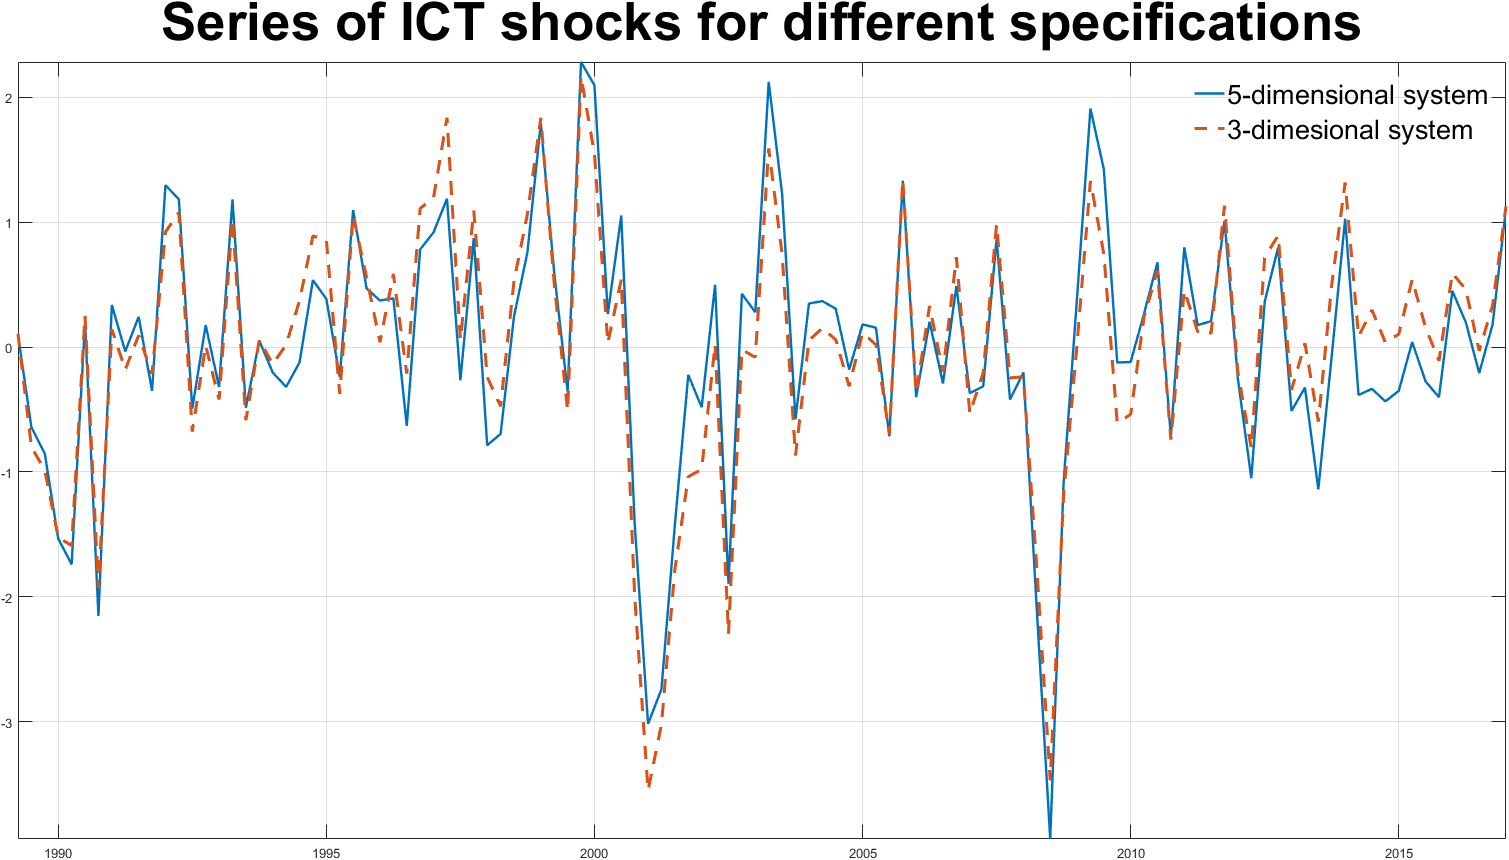
\includegraphics[scale=0.25]{Removing_FLVariables}
		\label{fig:TFP_main}
	\end{center}
\end{figure}


}

\frame{\frametitle{IRF Matching}


\

\begin{columns}[t]
\column{.3\textwidth}
\centering
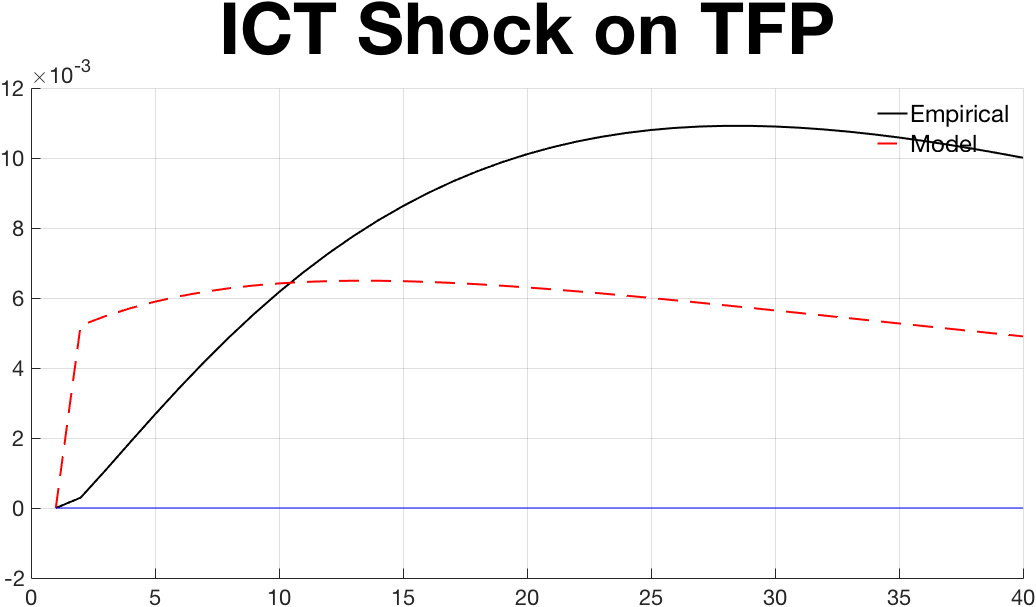
\includegraphics[width=4cm,height=3.5cm]{fig_ICT_Shock_on_TFP_IRmatching_together}\\
\bigskip
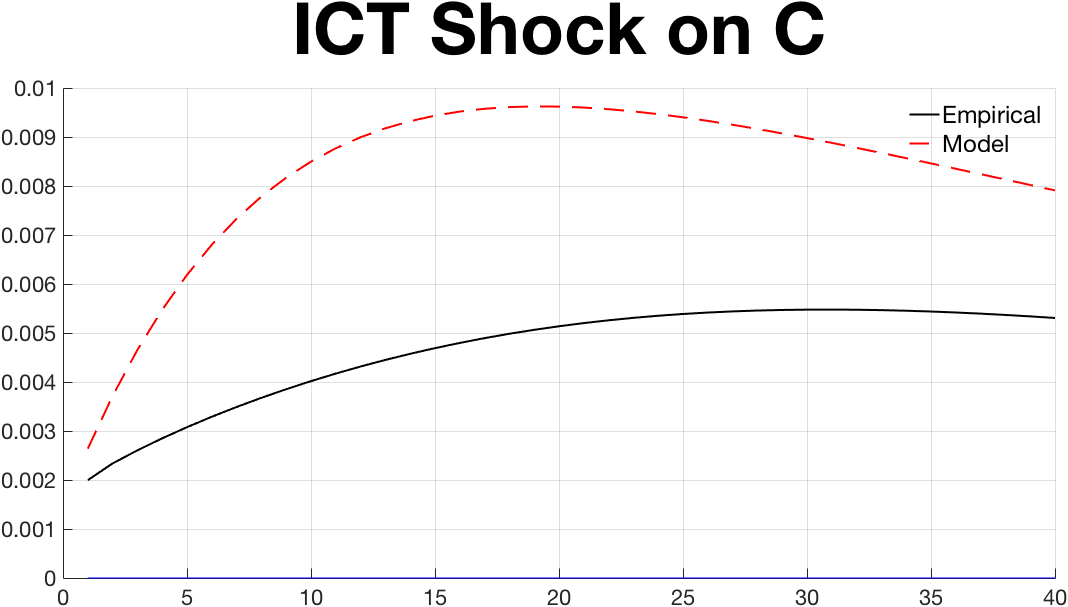
\includegraphics[width=4cm,height=3.5cm]{fig_ICT_Shock_on_C_IRmatching_together} 
\column{.3\textwidth}
\centering
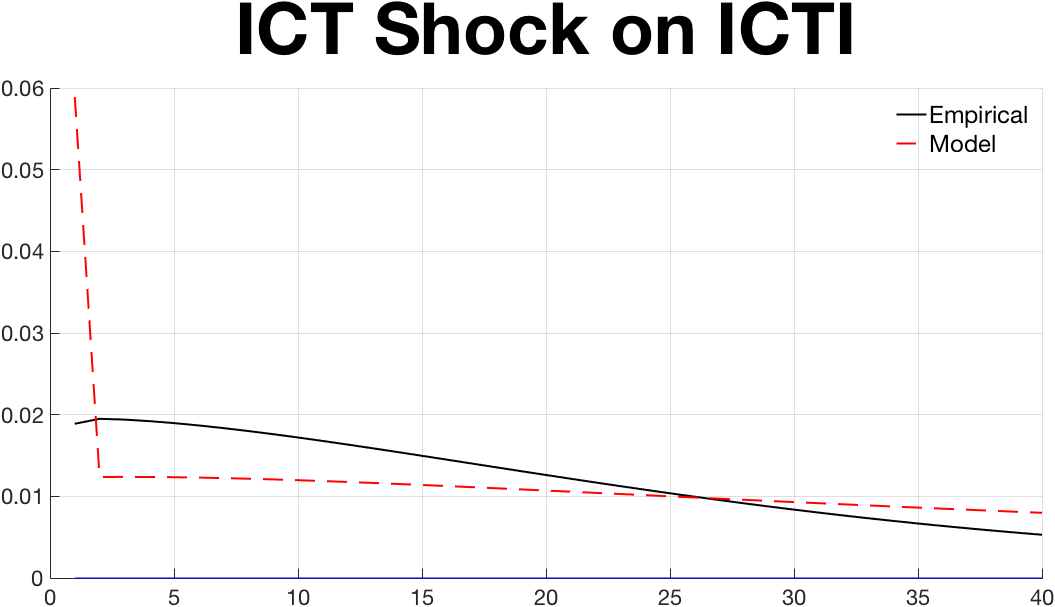
\includegraphics[width=4cm,height=3.5cm]{fig_ICT_Shock_on_ICTI_IRmatching_together}\\
\bigskip
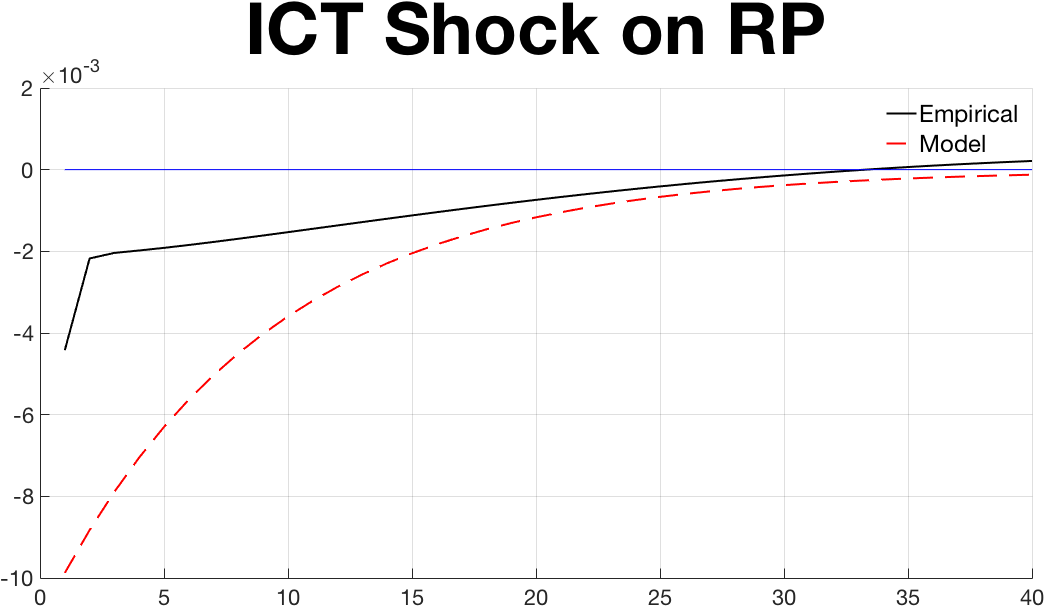
\includegraphics[width=4cm,height=3.5cm]{fig_ICT_Shock_on_RP_IRmatching_together}
\end{columns}







}




\end{document}